\documentclass[11pt]{article}
\usepackage{amsmath,amsthm,amssymb,fullpage,graphicx,hyperref,listings}
\usepackage{listings,color,setspace}
\author{Andy Reagan}
\title{Math 337 TEST 2}

     \def\NN{\mathbb{N} }
     \def\ZZ{\mathbb{Z} }
     \def\QQ{\mathbb{Q} }
     \def\RR{\mathbb{R} }
     \def\CC{\mathbb{C} }
     \def\f{\frac }
     \def\b{\begin }
     \def\e{\end }
     \def\Log{\text{Log} \,}
     \def\Re{\text{Re} \, }

\lstset{language=MATLAB,
basicstyle=\ttfamily\scriptsize\singlespacing,
keywordstyle=\color{blue},
stringstyle=\color{red},
commentstyle=\color{green},
morecomment=[l][\color{magenta}]{\#},
frame=L,
xleftmargin=\parindent,
%%numbers=left,                   %% where to put the line-numbers
%%numberstyle=\scriptsize,      %% the size of the fonts that are used for the line-numbers
%%stepnumber=1,                   %% the step between two line-numbers. If it is 1 each line will be numbered
numbersep=5pt,
breaklines=true,        %% sets automatic line breaking
breakatwhitespace=false,    %% sets if automatic breaks should only happen at whitespace
escapeinside={\%*}{*)} 
}


     \newcommand{\pdiff}[2]{\frac{\partial #1}{\partial #2}}
     \newcommand{\partialdiff}[2]{\frac{\partial #1}{\partial #2}}
     \newcommand{\pdiffsq}[2]{\frac{\partial^2 #1}{{\partial #2}^2}}
     \newcommand{\pdiffcu}[2]{\frac{\partial^3 #1}{{\partial #2}^3}}
     \newcommand{\pdiffhi}[3]{\frac{\partial^#3 #1}{{\partial #2}^#3}}
     \newcommand{\diff}[2]{\frac{{\rm d}#1}{{\rm d}#2}}
     \newcommand{\diffsq}[2]{\frac{{\rm d}^{2}#1}{{\rm d} {#2}^2}}
     \newcommand{\diffhi}[3]{\frac{{\rm d}^#3 #1}{{\rm d} {#2}^#3}}
     \newcommand{\tdiff}[2]{\mbox{d} #1/\mbox{d} #2}
     \newcommand{\tdiffsq}[2]{\mbox{d}^{2} #1/\mbox{d} {#2}^2}
     \newcommand{\tpdiff}[2]{\partial #1/\partial #2}
     \newcommand{\tpdiffsq}[2]{\partial^2 #1/\partial {#2}^2}
     \newcommand{\bvec}[1]{\vec{ {\bf #1 } }}
     \newcommand{\oh}[1]{O(h^{{#1}})}

\begin{document}
\maketitle

All of my code for each problem is included directly following that problem (no appendices for this one), since none is shared between problems.

\begin{enumerate}

\item (a) First I seek solutions to the homogeneous problem
\[ y'' + 10y = 0,\]
and to do so find roots of the characteristic equation
\[ r^2 + 10 = 0\]
which are $r = \pm i \sqrt{10}$.
Thus, we have the solutions for the homogeneous problem, which we can combine, such that we have
\[ y_h (x) = c_1 e^{i \sqrt{10} x } + c_2 e^{-i \sqrt{10} x}. \]
I use the variation of parameters method to find a particular solution:
\begin{align*} y_p &= -y_1 \int \f{y_2}{y_1y_2'-y_2y_1'}dx +y_2 \int \f{y_1}{y_1y_2'-y_2y_1'}dx\\
 &= -e^{i \sqrt{10} x } \int \f{e^{-i \sqrt{10} x }}{e^{i \sqrt{10} x }(e^{-i \sqrt{10} x })'-e^{-i \sqrt{10} x }(e^{i \sqrt{10} x })'}dx +e^{-i \sqrt{10} x } \int \f{e^{i \sqrt{10} x }}{e^{i \sqrt{10} x }(e^{-i \sqrt{10} x })'-e^{-i \sqrt{10} x }(e^{i \sqrt{10} x })'}dx\\
 &= -e^{i \sqrt{10} x } \int \f{e^{-i \sqrt{10} x }}{-2 \sqrt{10}}dx +e^{-i \sqrt{10} x } \int \f{e^{i \sqrt{10} x }}{-2 \sqrt{10}}dx\\
 &= -e^{i \sqrt{10} x } \left ( \f{e^{-i \sqrt{10} x }}{20}\right )  +e^{-i \sqrt{10} x }\left( \f{-e^{i \sqrt{10} x }}{20} \right )\\
 &= \f{1}{10}\end{align*}
Therefore, the general solution is
\[ y(x) = y_h + y_p = c_1 e^{i \sqrt{10} x } + c_2 e^{-i \sqrt{10} x}+\f{1}{10} .\]
Applying the boundary conditions, we have
\begin{align*} 0 &= c_1 + c_2 +\f{1}{10} \\
0 &= c_1 e^{i \sqrt{10} } + c_2 e^{-i \sqrt{10}}+\f{1}{10} \end{align*}
Solving the first equation for $c_1$, we plug $c_1 = -c_2 -1/10$ into the second equation
\[ 0 = (-c_2 -1/10) e^{i \sqrt{10} } + c_2 e^{-i \sqrt{10}}+\f{1}{10}~~~ \rightarrow~~~ c_2 = \f{-1/10 + 1/10 e^{i\sqrt{10}}}{e^{-i\sqrt{10}}-e^{i\sqrt{10}}}. \]

After all of this, I've noticed that both $\sin$ and $\cos$ are solutions to the homogeneous problem, so I'm going to try those to see if it works out nicer.
So we'll start with 
\[ y_h (x) = c_1 \cos (\sqrt{10} x) + c_2 \sin (\sqrt{10} x),\]
and we solve for the particular solution again, first observering that the Wronskian (the denominator in the integrals) is $\sqrt{10} \cos ^2 (\sqrt{10} x) + \sqrt{10} \sin ^2 (\sqrt{10} x) = \sqrt{10}$, so we have 
\begin{align*} y_p &= -y_1 \int \f{y_2}{\sqrt{10}}dx +y_2 \int \f{y_1}{\sqrt{10}}dx\\
&= -\cos (\sqrt{10} x) \int \f{\sin(\sqrt{10}x)}{\sqrt{10}}dx +\sin(\sqrt{10}x) \int \f{\cos (\sqrt{10} x)}{\sqrt{10}}dx\\
&= -\cos (\sqrt{10} x) \left ( \f{-\cos(\sqrt{10}x)}{10} \right )  +\sin(\sqrt{10}x) \left (  \f{\sin (\sqrt{10} x)}{10} \right ) \\
&= \f{1}{10}, \end{align*}
the same as before.
Now we have the general solution 
\[ y(x) = y_h (x) + y_p (x) = c_1 \cos (\sqrt{10} x) + c_2 \sin (\sqrt{10} x) + \f{1}{10},\]
and applying the boundary conditions we have the two equations for $c_{1,2}$:
\begin{align*} y(0) &= 0 = c_1 + \f{1}{10},\\
y(1) &= 0 = c_1 \cos (\sqrt{10}) + c_2 \sin (\sqrt{10}) + \f{1}{10},\end{align*}
so the first equation gives us that $c_1 = -1/10$ and we plug in for $c_2 = (-1/10-1/10\cos(\sqrt{10}))/\sin(\sqrt{10}) \approx 0.001$.

(b) Similarly, we have the same solution as above, but with all the 10's replaced with 9.9's.
That is, we have the homogeneous solution
\[ y_h (x) = c_1 \cos (\sqrt{9.9} x) + c_2 \sin (\sqrt{9.9} x),\]
and solve for the particular solution
\begin{align*} y_p &= -y_1 \int \f{y_2}{\sqrt{9.9}}dx +y_2 \int \f{y_1}{\sqrt{9.9}}dx\\
&= -\cos (\sqrt{9.9} x) \int \f{\sin(\sqrt{9.9}x)}{\sqrt{9.9}}dx +\sin(\sqrt{9.9}x) \int \f{\cos (\sqrt{9.9} x)}{\sqrt{9.9}}dx\\
&= -\cos (\sqrt{9.9} x) \left ( \f{-\cos(\sqrt{9.9}x)}{9.9} \right )  +\sin(\sqrt{9.9}x) \left (  \f{\sin (\sqrt{9.9} x)}{9.9} \right ) \\
&= \f{1}{9.9}, \end{align*}
The general solution is thus
\[ y(x) = y_h (x) + y_p (x) = c_1 \cos (\sqrt{9.9} x) + c_2 \sin (\sqrt{9.9} x) + \f{1}{9.9},\]
Solving for $c_{1,2}$, we get $c_1 = -1/9.9$ and we plug in for $c_2 = (-1/9.9-1/9.9\cos(\sqrt{9.9}))/\sin(\sqrt{9.9}) \approx 41.7924$.

Here is a plot:

\begin{figure}[h!]
  \centering
    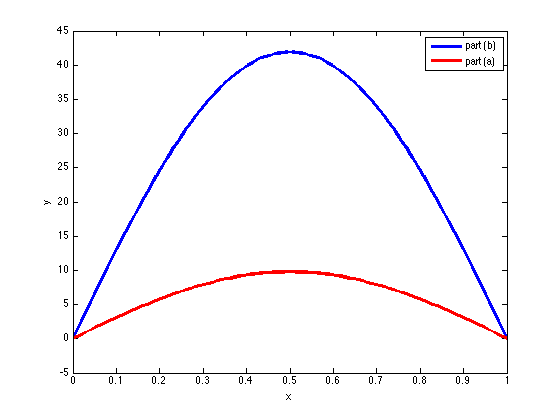
\includegraphics[width=0.5\textwidth]{andy_exam02_prb01_01.png}
  \caption{Numerical and analytical solution to the BVP using the shooting method.}
\end{figure}

The reason that these solutions are so different is that in calculating $c_2$ on for part (b) on the computer, two numbers that are very close in magnitude are subtracted. Namely, $\cos(\sqrt{9.9}) \approx \cos (\pi) = -1$, so we have $(-1/9.9+1/9.9)$ on the top where the second number is not quite 1/9.9, but very close.
This small number is then magnified by dividing by $\sin(\sqrt{9.9})$, which is very close to 0.

\lstinputlisting[language=Matlab]{andy_exam02_prb01.m}


\item First, I write the second order ODE as a system of two first-order ODEs by letting $u' = v$ and therefore $v' = u'' = \f{x-6+2u}{x^2}$.
I shoot twice, first with the nonhomogeneous system as the IC $u = 0, v = u'(2) = -15/19$, call this solution $h$.
The second shot is with the homogeneous system, starting with $u=1, v = 0$ such that any multiple of this solution is still a solution, and will have $u' = 0$.
Therefore, the solution to the BVP is
\[ w = h + \theta z ~~~\Rightarrow ~~~\theta = (u(3)-h(3))/z(3) = -h(3)/z(3).\]
The following code implements this solution, plotting both the error in $u$ and $u'$.
We observe that the error in $u$ is 0 at $x = 3$, satisfying the Dirichlet BC, and that the error in $u'$ at $x=2$ is zero, satisfying the Neumann BC.

\begin{figure}[h!]
  \centering
    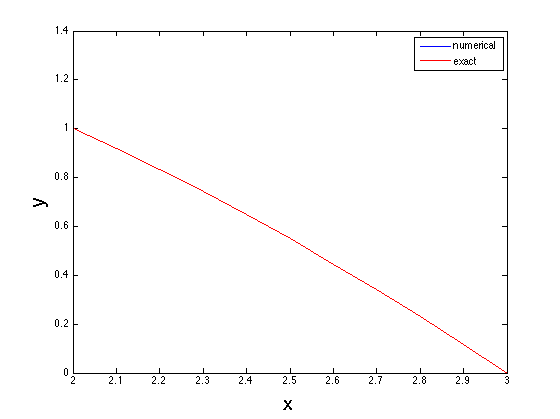
\includegraphics[width=0.5\textwidth]{andy_exam02_prb02_01.png}
  \caption{Numerical and analytical solution to the BVP using the shooting method.}
\end{figure}

\begin{figure}[h!]
  \centering
    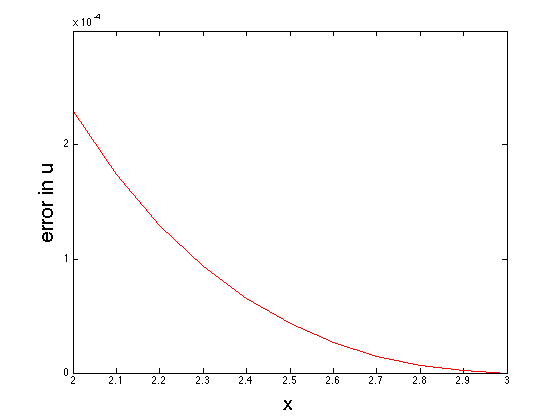
\includegraphics[width=0.5\textwidth]{andy_exam02_prb02_02.png}
  \caption{Error in $u$ of the numerical solution.}
\end{figure}

\begin{figure}[h!]
  \centering
    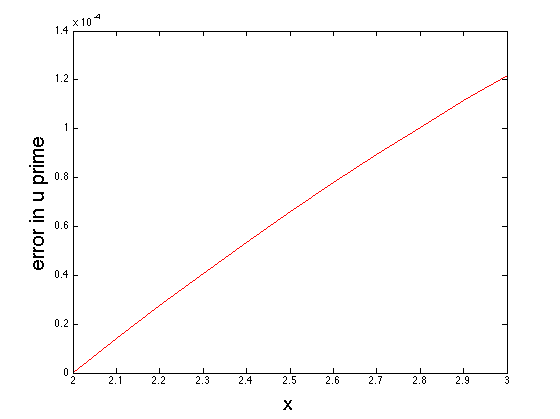
\includegraphics[width=0.5\textwidth]{andy_exam02_prb02_03.png}
  \caption{Error in $u'$ of the numerical solution.}
\end{figure}

\lstinputlisting[language=Matlab]{andy_exam02_prb02.m}
\lstinputlisting[language=Matlab]{andy_ME.m}
\lstinputlisting[language=Matlab]{andy_exam02_prb02_ODE.m}
\lstinputlisting[language=Matlab]{andy_exam02_prb02_ODEh.m}


\clearpage
\pagebreak
\item I solve the same problem as above using the second-order finite difference scheme, chapter 8 of the notes.

I use method 1 of section 8.4 to handle the Neumann BC.
In equation 8.36, there is no modification to the $Y_0$ term since $A_1 = 0$, and the $Y_1$ term needs an extra 1. In the code, I just add $[0,1]$ to the top of the matrix $A$.
In $R$, the first entry is adjusted from Eq 8.7 by subtracting $2h\alpha /A_2$ per Eq 8.36 as well.

I include the code and my plot of the solution (and exact), as well as the error.

\begin{figure}[h!]
  \centering
    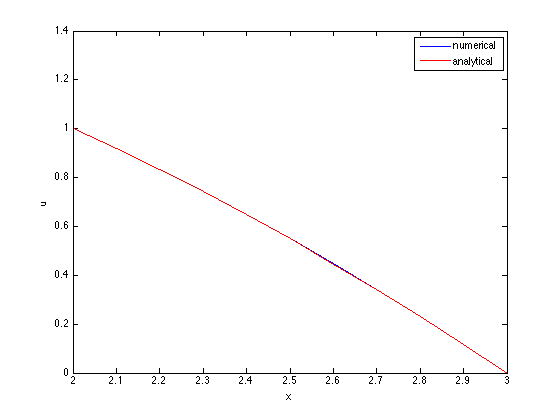
\includegraphics[width=0.5\textwidth]{andy_exam02_prb03_01.png}
  \caption{Numerical and analytical solution to the BVP using the second-order finite difference method.}
\end{figure}

\begin{figure}[h!]
  \centering
    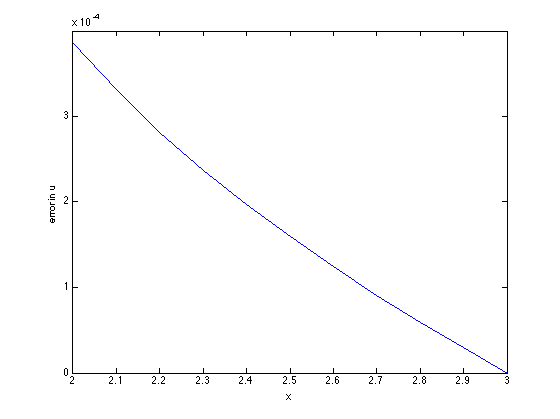
\includegraphics[width=0.5\textwidth]{andy_exam02_prb03_02.png}
  \caption{Error in $u$ of the numerical solution.}
\end{figure}

\lstinputlisting[language=Matlab]{andy_exam02_prb03.m}

\item I use the Newton-Raphson method, based on the results of the homework assignments. Convergence is obtained for each solution in 9 iterations.

Applying NR to this BVP, the discrete equation for error is found by plugging $Y_n = Y_n ^{(0)} - \epsilon _n ^{(0)}$ into the discretize problem:
\[ Y_{n+1} -2 Y_n + Y_{n-1} = h^2 Y_n \left [ Y_n ^2 + \lambda - 6 \text{sech}^2 x_n \right ] .\]
Bringing all of the terms in $\epsilon^{(0)}$ to the RHS, and dropping terms of order greater than and including $\left (\epsilon _n ^{(0)}\right ) ^2$, we are left with a linear equation in $\epsilon^{(0)}$:
\begin{align*} &Y^{(0)}_{n+1} -2 Y_n ^{(0)} + Y_{n-1}^{(0)} - h^2 Y_n ^{(0)} \left [ \left ( Y_n ^{(0)} \right ) ^2 + \lambda - 6 \text{sech}^2 (x_n) \right ]\\
&~~~~=\epsilon^{(0)}_{n+1} -2 \epsilon _n ^{(0)} + \epsilon _{n-1}^{(0)} + \epsilon _n ^{(0)} \left [ -3 \left ( Y_n ^{(0)} \right ) ^2 -\lambda + 6 \text{sech}^2 (x_n ) \right ] \end{align*}

\begin{figure}[h!]
  \centering
    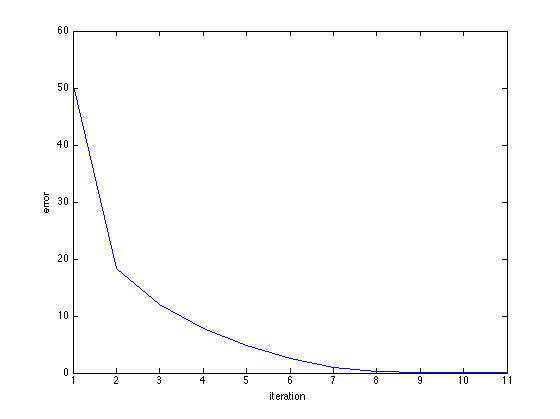
\includegraphics[width=0.5\textwidth]{andy_exam02_prb04_01.png}
  \caption{Error versus iteration count for Newton-Raphson applied to the nonlinear BVP with $\lambda = 2.25$ and initial function $e^{-x^2}$.}
\end{figure}

\begin{figure}[h!]
  \centering
    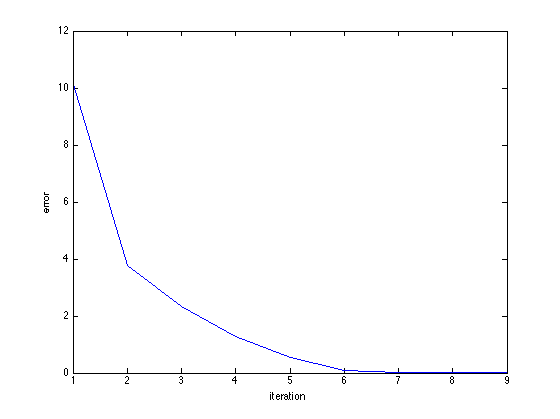
\includegraphics[width=0.5\textwidth]{andy_exam02_prb04_02.png}
  \caption{Error versus iteration count for Newton-Raphsonapplied to the nonlinear BVP with $\lambda = 0.778$ and initial function $xe^{-x^2}$.}
\end{figure}

\lstinputlisting[language=Matlab]{andy_exam02_prb04.m}
\lstinputlisting[language=Matlab]{andy_exam02_prb04_r.m}

\end{enumerate}

%% \begin{figure}[h!]
%%   \centering
%%     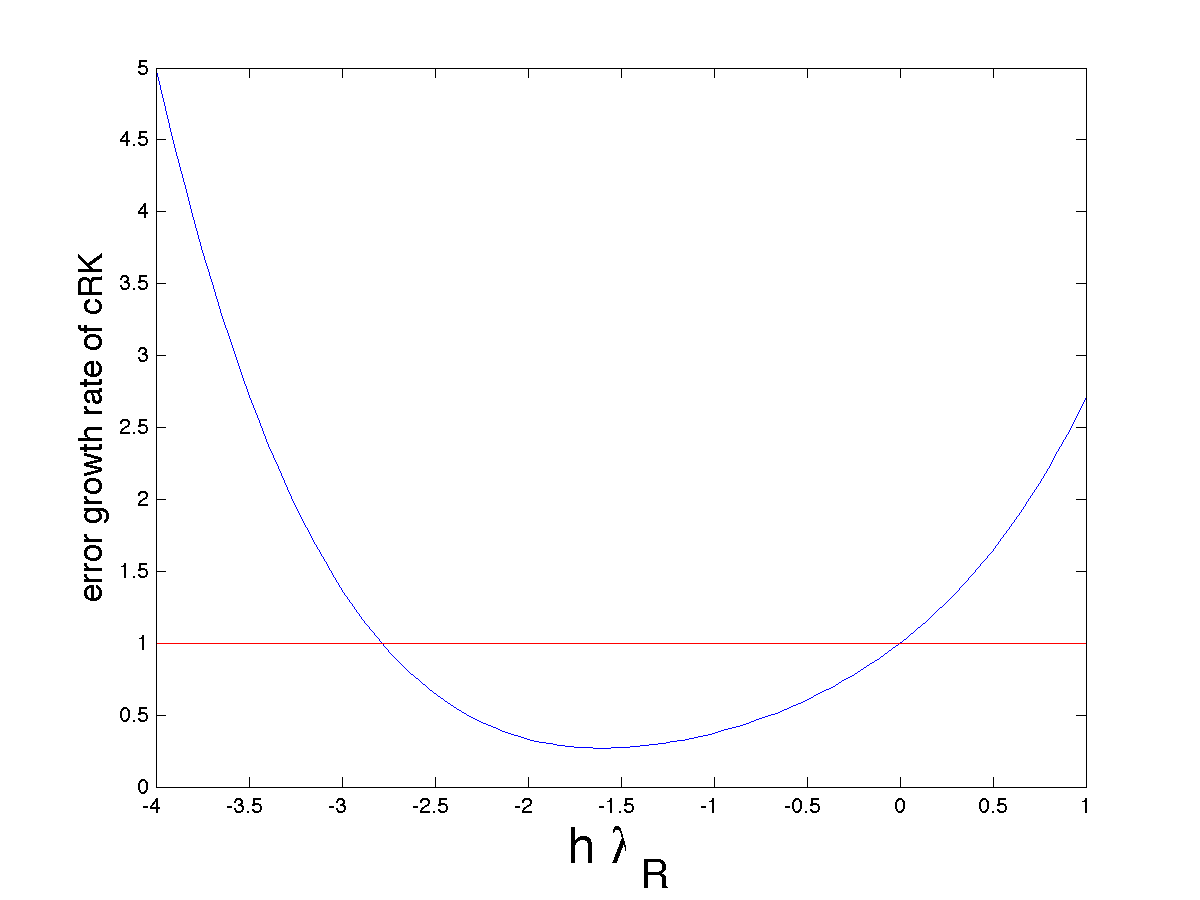
\includegraphics[width=0.5\textwidth]{andy_hw04_prb02_01.png}
%%   \caption{Stability of the cRK method.}
%% \end{figure}

%% \lstinputlisting[language=Matlab]{andy_hw04_prb04.m}

\end{document}
